\subsection{Five step approach}
A serial-link manipulator consists of links in a chain connected by joints. 
%A link is a rigid body, defining the spatial relationship between two following axes. %Glossary
For describing the serial-link mechanism geometry the Denavit Hartenberg notation is one possible approach.
It gives a description of a manipulator for kinematic solutions, Jacobians, dynamics, motion planning and simulation. 
This description can be obtained through a five step algorithm:\cite{ConstantinForwardKA}

\begin{enumerate}
	\item Numbering of joints and links
	\item Set up local coordinate reference frames
	\item Establishing \ac{DH} parameters for each link
	\item Calculate homogeneous transformation matrices
	\item Compute Forward Kinematic Equations
\end{enumerate}

\subsubsection{Numbering of joints and links} \label{sec:NumJointLink}
A serial link robot with n joints has $n+1$ links. 

\paragraph{numbering of links}
The numbering scheme for links starts at $(0)$ with the fixed grounded base and then increases sequentially up to $(n)$ for the end effector.

\paragraph{numbering of joints}
The numbering scheme for joints starts at $(1)$ with the joint connecting the first movable link to the base and then increases sequentially up to n.

\paragraph{relation between links and joints}
Link $(i)$ is connected to its 
\begin{itemize}
	\item lower link $(i-1)$ at its proximal \cite{proxdist} end by joint $(i)$
	\item upper link $(i+1)$ at its distal \cite{proxdist} end by joint $(i+1)$
\end{itemize}



\subsubsection{Set up local coordinate reference frames} \label{sec:localRefFrame}
With the Denavit-Hartenberg convention, local coordinate frames can be attached to the far end of the links $ (i) $ and their accompanying joints $ (i+1) $.
Each link $(i)$ is described relative to the pose of the preceding link.

%\paragraph{Assignation of coordinate frames}


\paragraph{Assignation of $z_i$ axes}\label{par:z_iAxesAssign}

With the DH-notation, the $z_i$ axes are assigned to link $(i)$. 
By using the  DH convention, both prismatic and revolute joints can be treated similarly: %regarding joint $(i+1)$:
\begin{itemize}[wide=\parindent]
	\item[\textbf{revolute:}] $z_i$ is the axis of revolution of joint $(i+1)$
	\item[\textbf{prismatic:}] $z_i$ is the axis of translation of joint $(i+1)$
\end{itemize}
%of joint $(i+1)$
This means, that joint $z_i$ turns around axis $z_i$.

\paragraph{Direction of rotation}
With the direction of the $z_i$-axis, the direction of positive rotation around joint $(i+1)$ is also given by the right hand rule (see \cite{RightHandRule} and \cite{Angela_U1S2P1} at 10:35 for a visual representation). This means, the direction of positive rotation is counter-clockwise around the $z_i$-axis.
With predictive choice of the direction of positive rotation, the direction of the z-axis can be chosen in order to minimize the DH-parameters (insert source here)



\paragraph{Base frame}

The base frame $(0)$ can be chosen nearly arbitrarily. The origin of the base frame can be any point on $z_0$. For simplicity, the origin of frame$(0)$ can be put into joint$(1)$.  Usually, the x-axis of the base frame is chosen, so that it points in the direction of the \ac{EOAT} in default position according to its base, \cite{DenavitHartenbergKonventionen} but can be chosen in any convenient manner \cite{SpongDynContr}.

\paragraph{Assignation of frames $(i)$}

Starting from frame $(1)$ in an iterative process, frame $(i)$ can be set up using frame $(i-1)$.

Three cases regarding the relationship of axes $z_{i-1}$ and $z_i$  need to be considered when setting up frames:
\begin{itemize}[wide=\parindent] %option solves alignment problem for item label %https://tex.stackexchange.com/questions/246394/alignment-of-labels-in-itemize-with-text-of-document 
	\item[\textbf{Non coplanar:}] Axes don't intersect and are not parallel. Line containing the common normal $z_{i-1}$ to $z_i$ defines $x_i$-axis and the point of intersection with $z_i$ is the origin of frame $(i)$
	\begin{enumerate}[label=\emph{\alph*)}]
		\item find common normal of the joint axes
		\item put origin in intersection of normal with joint axis
		\item put $z_i$ axis in the joint axis
		\item $x_i$ points in direction of the common normal, facing away from frame $(0)$
		\item add $y_i$ according to right hand rule
	\end{enumerate}
	\item[\textbf{Parallel:}] Axes are parallel. Line containing the normal through origin of frame $(i+1)$ and the $z_i$-axis defines the $x_i$-axis which is directed from origin of frame $(i)$ toward the distal joint. The point of intersection of common normal with $z_i$-axis gives the origin of frame $(i)$. % found a mistake here with common normal in \cite{ConstantinForwardKA} witht he help of \cite{SpongDynContr}. The x-axis should point towards next joint, but he says, should point towards last joint, but does it actually the other way around.
	\begin{enumerate}[label=\emph{\alph*)}]
		\item look for normal originating from distal joint
		\item put origin in the intersection of the normal with the joint axis
		\item put the $z_i$ axis in the joint axis of the link $(i+1)$ 
		\item $x_i$ points follows the common normal with the distal joint, pointing towards the distal joint
		\item add $y_i$ according to right hand rule
	\end{enumerate}
	\item[\textbf{Intersecting:}] Axes are intersecting. Line containing the normal to the plane formed by axes $z_{i-1}$ and  $z_i$ gives the $x_i$-axis with positive direction chosen arbitrarily. Point of intersection of  axes $z_{i-1}$  and  $z_i$ is the origin of frame $(i)$.
	\begin{enumerate}[label=\emph{\alph*)}]
		\item put origin in intersection point of the axes
		\item put the $z_i$ axis in the joint axis of the link $(i+1)$
		\item $x_i$ is perpendicular to both joint axes
		\item add $y_i$ according to right hand rule
	\end{enumerate}
\end{itemize}

\paragraph{Assignation of \ac{EOAT} frame}
As there is no distal joint for the \ac{EOAT} frame, the steps for this frame are different:

\begin{enumerate}[label=\emph{\alph*)}]
	\item put origin on axis of proximal joint 
	\item axis $z_i$ follows direction of $z_{i-1}$
	\item $x_i$ can be chosen arbitrarily, but is usually determined by screw holes
	\item add $y_i$ according to right hand rule
\end{enumerate}


\subsubsection{Establishing \ac{DH} parameters for each link} \label{sec:DHparPerLink}

After assigning the local coordinate frames, the \ac{DH}-Transformations to connect the coordinate frames have to be determined according to \ac{DH}-convention.
Further notes on the \ac{DH}-convention can be found in \fullref{sec:DH-convention}.




The \ac{DH}-parameters form the transformation matrices that connect serial link coordinate frames. They can be distinguished into parameters and variables. While constructive parameters are dependent on the construction of the robot and are constant, variables depend on the joint movement \cite{FwdInvAnalysRobManip} \cite{ConstantinForwardKA} \cite{DenavitHartenbergKonventionen}.

\begin{enumerate}[label=\emph{\arabic*)}]
	\item[$\alpha_i$] angle between $z_{i-1}$ and $z_i$, measured in plane normal to $x_i$ (constructive parameter)
	\item[$a_i$] distance between $z_{i-1}$ and $z_i$, measured along $x_i$; parallel to $z_{i-1} \times z_i$ for intersecting axes (constructive parameter)
	\item[$d_i$] distance from the origin $O_{i-1}$ of frame $i-1$ to the intersection of the $x_i$ axis with $z_{i-1}$, measured along $z_{i-1}$ (constructive parameter in revolute joints, variable in prismatic joints)
	\item[$\theta_i$] angle between $x_{i-1}$ and $x_i$, measured in plane normal to $z_{i-1}$ (constructive parameter in prismatic joints, variable in revolute joints)
\end{enumerate}

These parameters describe the relatively complex transformation of the coordinate system $i-1$ into the coordinate system $i$ by four subsequent elementary transformations \cite{allgInvKin}:

\begin{equation} \label{eq:DH-Transform}
T_{i-1,i}=ROT(z_{i-1}, \theta_i) * TRANS(0,0,d_i)^T * TRANS(a_i,0,0)^T * ROT(x_i,\alpha_i)
\end{equation}

$ROT(v,\alpha)$ is a simple rotation around vector $v$ with the angle $\alpha$ and $TRANS(x,y,z)^T$ is a translational movement along the vector $[x,y,z]^T$. For a visual representation of these parameters see figure \ref{fig:DH_Parameters_visual} 

\begin{figure}[H]
	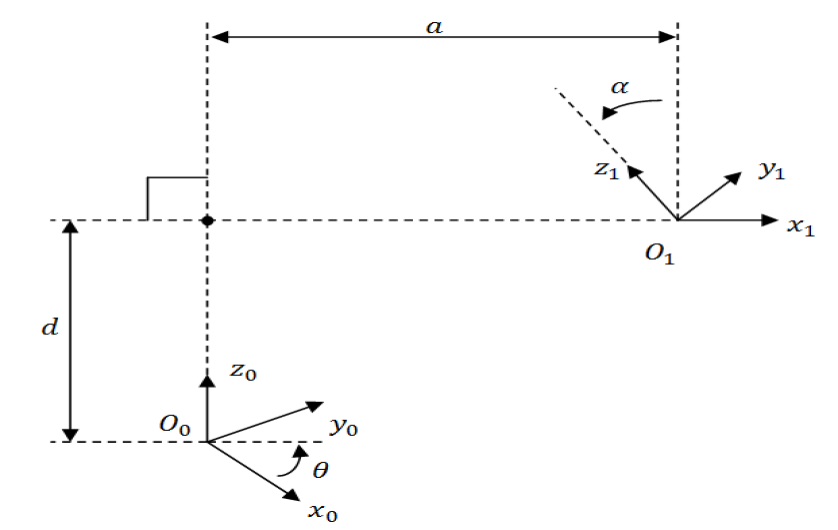
\includegraphics[
	width=0.8\linewidth,
	center,
	keepaspectratio,
	]{coordinateFrames/DH_Parameters_visual}
	\caption{Visual representation of a \ac{DH}-transformation}
	\label{fig:DH_Parameters_visual}
\end{figure}

This visual representation gives a guide to attach the \ac{DH}-parameters on serial-link mechanisms.


\subsubsection{Calculate homogeneous transformation matrices}

Locating reference frame $(i-1)$ relative to $(i)$ can be done by executing a series of transformations as given by equation \ref{eq:DH-Transform}. 
For simplification, they can be done with a 4 × 4 homogenous transformation matrix:
\begin{equation} \label{eq:fourTransformations}
^{i-1}T_i(\theta_i,d_i,a_i,\alpha_i)=R_z(\theta_i)*T_z(d_i)*T_x(a_i)*R_x(\alpha_i)
\end{equation}
Equation \ref{eq:fourTransformations} can be expanded into:
\begin{equation}\label{eq:TransformationMarix}
^{i-1}T_i=
\begin{bmatrix}
\cos\theta_i & -\sin\theta_i*\cos\alpha_i & \sin\theta_i*\sin\alpha_i & a_i*\cos\theta_i \\
\sin\theta_i & \cos\theta_i*\cos\alpha_i & -\cos\theta_i*\sin\alpha_i & a_i*\sin\theta_i \\ %Typo in source column 3 - source used cos instead of sin alpha_i
0 & \sin\alpha_i & \cos\alpha_i & d_i \\
0 & 0 & 0 & 1 \\
\end{bmatrix}
\end{equation}



\subsubsection{Compute Forward Kinematic Equations} \label{ForKinEq}
In Forward kinematics, the kinematic equations of a robot are used to compute the position of the \ac{EOAT} from the given joint parameters.

\paragraph{Sum of Transformations Matrix}
With the transformation matrices from frame $(i)$ to $(i-1$), a $4×4$ matrix for all joints on n links can be established as in equation \ref{eq:SummofTranfMatr}

\begin{equation} \label{eq:SummofTranfMatr}
^0T_n=\prod_{n}^{i=1} \phantom{.}^{i-1}T_i
\end{equation}


The resulting matrix has the form (see \cite{invKinSolYanWu}, eq 1):
\begin{equation}\label{eq:matrixForm}
^0T_n=
\begin{bmatrix}
n & o & a & p \\
0 & 0 & 0 & 1 \\
\end{bmatrix}
=
\begin{bmatrix}
n_x & o_x & a_x & p_x \\
n_y & o_y & a_y & p_y \\ %mistake here in source?\cite{invKinSolYanWu} xyz broken? - error confirmed!
n_z & o_z & a_z & p_z \\
0 & 0 & 0 & 1 \\
\end{bmatrix}
\end{equation}

\paragraph{short notation}
The short notations for orientation, rotation and position are defined as:

\begin{itemize}
	\item[n] normal vector
	\item[o] orientation vector
	\item[a] approach vector
	\item[p] position
\end{itemize}


\paragraph{Transformation to cartesian coordinates with euler angles }
These vectors can be transformed into the $[x,y,z,\alpha,\beta,\gamma]$ notation.
Vector $p = [p_x, p_y, p_z] $ gives [x, y,z].
The rotational approach $[\alpha, \beta, \gamma]$ can be calculated with the rotation matrix R as seen in eq \ref{eq:rotMatrix_composition}.
\begin{equation}\label{eq:rotMatrix_composition}
T = 
\begin{bmatrix}
R & p \\
0 & 1 \\
\end{bmatrix}
\end{equation}

The rotation matrix describes the relative orientation of two frames towards each other. As the columns $[n,o,a]$ are the unit vectors along the axes of one frame relative to the other reference frame, the relative orientation of a frame ${b}$ with respect to a frame ${a}$ is given by the rotation matrix as seen in eq \ref{eq:rotMatrix_a-b} \cite{ConstantinForwardKA}
\begin{equation}\label{eq:rotMatrix_a-b}
\phantom{}^b_aR =
\begin{bmatrix}
\phantom{}_ax^b) & \phantom{}_ay^b) & \phantom{}_az^b) \\
\end{bmatrix}
=
\begin{bmatrix}
x^b \cdot x^a & y^b \cdot x^a & z^b \cdot x^a \\
x^b \cdot y^a & y^b \cdot y^a & z^b \cdot y^a \\
x^b \cdot z^a & y^b \cdot z^a & z^b \cdot z^a \\
\end{bmatrix}
\end{equation}

The coordinates relative to the reference frame ${a}$, of a point $p$, of which the coordinates are known with respect to a frame ${b}$ with the same origin can then be calculated as in equation \ref{eq:rotMatrixToAbsFrame}  ( see \cite{RobotKinemDyn}, "Description of Position and Orientation) .
\begin{equation}\label{eq:rotMatrixToAbsFrame}
\phantom{}_a p = \phantom{}^b_aR\phantom{.}_b p 
\end{equation}


